\documentclass[a4paper,10pt]{article}
\usepackage[utf8]{inputenc}
\usepackage{graphicx}
\usepackage{float}

\title{Detecting contours of human organs in CT images using the Marr-Hildreth edge detector}
\author{Neža Belej (63120340)}

\begin{document}

\maketitle
\section {Abstract}
In the following report we represent our program for edge detection in CT images of human organs. We achieve this by using Marr-Hildreth algorithm. We use images from CTMRI database \cite{db}. In the end, we discuss the advantages and disadvantages of Marr-Hildreth algorithm and propose possible improvements.
\section{Introduction}
Edge detection is one of the most commonly used operations in image analysis. An edge is defined by a
discontinuity in gray level values. In other words, an edge is the boundary between an object and the background \cite{article1}. Most popular edge detecting algorithms are The Marr-Hildreth Edge Detector, The Canny Edge Detector, The Local Threshold and Boolean Function Based Edge Detection, Color Edge Detection Using Euclidean Distance and Vector Angle. \cite{article2}
\\
We used Marr-Hildreth edge detector and tested it on CTMRI database. We obtained the images with \textit{wget} command: \\

\textit{sudo wget -r --no-parent --user=bsip --ask-password \\ http://lbcsi.fri.uni-lj.si/OBSS/Data/CTMRI/Images-Patient-000302-01/}

\section{Methods}

We used Marr-Hildreth edge detection algorithm. The steps are following:
\begin{enumerate}
\item{Calculate coefficients of the LoG operator (mask).}
\item{Apply this mask on the image to enhance edges.}
\item{Searching for zero crossings and perform binarization.}
\end{enumerate}

Zero crossings are the key feature of the Marr-Hildreth edge detection method. For every pixel p:
\begin{itemize}
\item{we use a 3 x 3 neighborhood centered at p,}
\item{ the signs of at least two of opposing neighboring pixels of a pixel p considered must differ (there are four cases: left/right, up/down, and the two diagonals),}
\item{ the absolute value of their numerical differences must exceed the threshold T.}
\end{itemize}

\section{Results}
We tested our algorithm on the CT images of CTMRI database. Results show that edge detector successfully detects edges. It finds the correct places of edges, but the edges are not always thin and they are too spotty.\\
Our input images are in the folder /input/. We tested our images with 2 different masks: one is dynamic, obtained from image size properties; the second mask is smaller and static. We stored output images, obtained with first mask, in folder /output/; the second is in /output2/. We see from results how much effect has the filter on the output image.
We also tested the effect of the threshold, used in zero crossing.
Example:
\begin{figure}[H]
  \caption{Input image.}
  \centering
    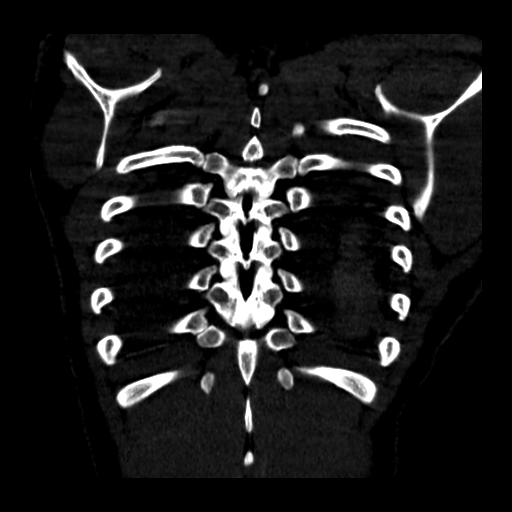
\includegraphics[width=0.7\textwidth]{0099.png}
\end{figure}

\begin{figure}[H]
  \caption{Output image, threshold = 0, dynamic mask.}
  \centering
    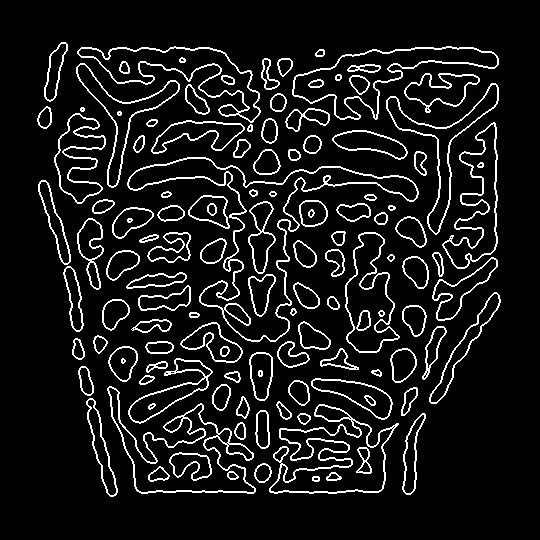
\includegraphics[width=0.7\textwidth]{out.png}
\end{figure}

\begin{figure}[H]
  \caption{Output image, threshold = 0, small static mask.}
  \centering
    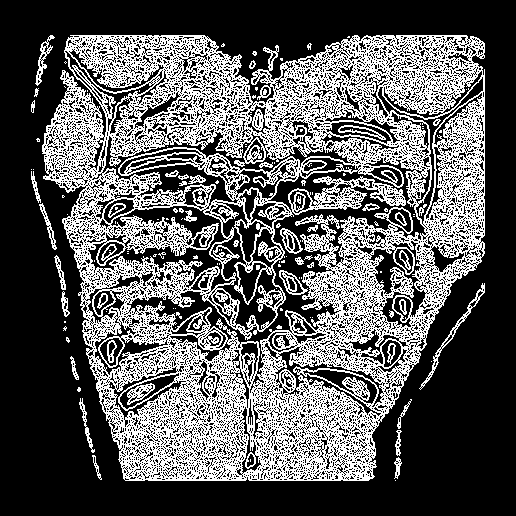
\includegraphics[width=0.7\textwidth]{out2.png}
\end{figure}

\begin{figure}[H]
  \caption{Output image, threshold = 2, small static mask.}
  \centering
    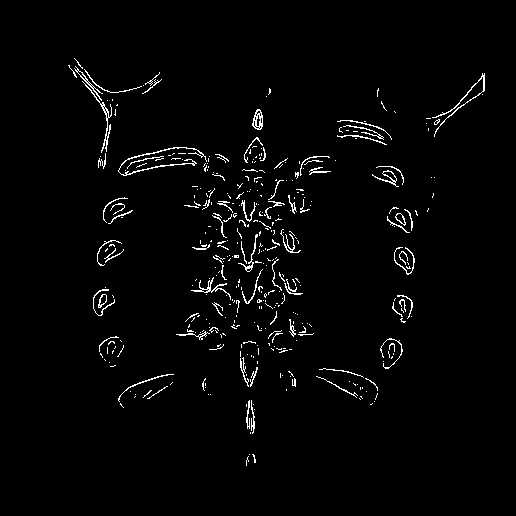
\includegraphics[width=0.7\textwidth]{out3.png}
\end{figure}

\begin{figure}[H]
  \caption{Output image, obtained with built-in function.}
  \centering
    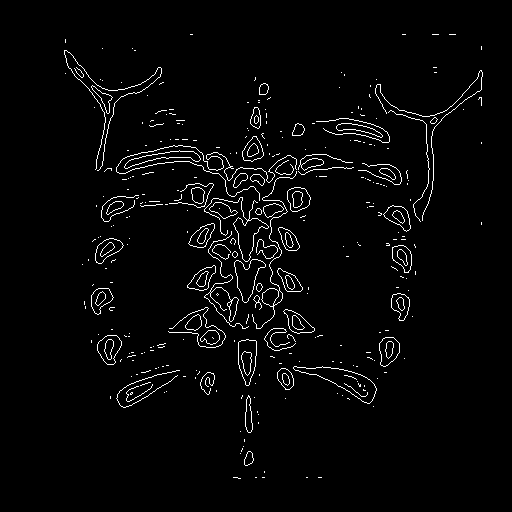
\includegraphics[width=0.7\textwidth]{out4.png}
\end{figure}

\section{Discussion}
The MarrHildreth detector perceives many edges, but they are too spotty and wide to really
identify any features. In Marr-Hildreth, locality is not especially good and the edges are not always thin. \\
We could improve our edge detection with using Canny Edge Detector, which is more accurate and good with locality.
We could also combine different parameters (sigma and threshold in zero crossing) to get the best effect.
\begin{thebibliography}{9}

\bibitem{article1}
 Sharifi, Mohsen and Fathy, Mahmood and Mahmoudi, Maryam Tayefeh,
  \emph{A classified and comparative study of edge detection algorithms},
  Information Technology: Coding and Computing, 2002. Proceedings. International Conference on, IEEE,
  2002.
\bibitem{article2}
 Ehsan Nadernejad, Sara Sharifzadeh : 
  \emph{Edge Detection Techniques: Evaluations and Comparisons},
  Applied Mathematical Sciences, Vol. 2, 2008, no. 31, 1507 - 1520 
\bibitem{db}
  \emph{http://lbcsi.fri.uni-lj.si/OBSS/Data/CTMRI/}


\end{thebibliography}

\end{document}

